% !TeX root = ../main.tex

\chapter{Standard Model}

The Standard Model (SM) is the theory which describes the interactions between fundamental particles 
(which are listed in table~\ref{table:pdg-table}).
As far as we know, the interactions between fundamental particles are just four: \textit{Gravitational}, 
\textit{Electromagnetic}, \textit{Weak} and \textit{Strong}.\footnote[1]{The Higgs boson interaction
can be considered as the fifth interaction of Nature. A particle acquires mass by interacting with the Higgs' 
field.}
The SM is a non-Abelian Gauge theory whose symmetry group is:

\begin{equation}
    SU(3) \times SU(2) \times U(1)
\end{equation}

In reality this statement is unprecise, since what we know is only the Lie algebra of the SM.%
\footnote{
    An introduction to Group Theory is beyond the scope of this brief introduction to the SM, 
    but to not leave the reader completely dissatisfied with this statement, 
    what I will limit myself to say is that different groups share the same algebra, so having access only 
    to the algebra, we cannot uniquely determine the underlying group.}

This theory consists of two main sectors: Quantum Chromodynamics (QCD), which describes the Strong interaction 
and is based on the $SU(3)$ symmetry, and the Electroweak sector (EW), which desccribes the Weak 
and Electromagnetic interactions and is based on the $SU(2) \times U(1)$ symmetry.\\
The SM does not offer a proper description of \textit{Gravity}, it only suggests the existence of 
the \textit{Graviton}, the mediator of the gravitational interaction.
However, this particle has not been discovered thus far, therefore a completely satisfactory quantum 
theory of gravity has yet to be formulated.\\

\begin{table}[h]
    \centering
    \begin{tabular}{ccccc}
    \toprule
    & Particle & Mass (MeV) & Mean Life (s) & Charge (e) \\
    \midrule
    \multirow{4}{*}{Leptons} & $e^-$ & $0.511 \pm 10^{-9}$ & $> 6.6 \times 10^{28}$ yr &  \\
    & $\mu^-$ & $105.7 \pm 10^{-6}$ & $2.197 \times 10^{-6}$ & $-1$  \\
    & $\tau^-$ & $1776.86 \pm 0.12$ & $(290.3 \pm 0.5) \times 10^{-15}$ &  \\
    & $\nu_e, \nu_{\mu}, \nu_{\tau}$ & $< 2 \times 10^{-6}$ & - & $0$  \\
    \midrule
    \multirow{6}{*}{Quarks} & $u$ & $2.16^{+0.49}_{-0.26}$ & - &   \\
    & $c$ & $(1.27 \pm 0.02) \times 10^3$ & - & $\frac{2}{3}$  \\
    & $t$ & $172.69 \pm 0.30 \times 10^3$ & - &   \\
    & $d$ & $4.67^{+0.48}_{-0.17}$ & - &    \\
    & $s$ & $93.4^{+8.6}_{-3.4}$ & - & $-\frac{1}{3}$  \\
    & $b$ & $(4.18^{+0.03}_{-0.02}) \times 10^3$ & - &   \\
    \midrule
    & Particle & Mass (GeV) & Decay Width (GeV) & Charge (e) \\
    \midrule
    \multirow{5}{*}{Bosons} & $\gamma$ & $< 10^{-24}$ & Stable & $< 10^{-35}$  \\
    & $W^{\pm}$ & $80.379 \pm 0.012$ & $2.197 \times 10^{-6}$ & $\pm 1$  \\
    & $Z^0$ & $91.1876 \pm 0.0021$ & $2.4952 \pm 0.0023$ & $0$  \\
    & $g$ & $0$ & - & $0$  \\
    & $H$ & $125.18 \pm 0.16$ & $< 0.013$ & $0$  \\
    \bottomrule
    \end{tabular}
    \caption{Properties of the Standard Model Particles as given by the PDG~\cite{pdg}.}
    \label{table:pdg-table}
\end{table}

As part of this introduction to the SM, before discussing in detail the main 
two sectors of the SM, I believe it is instructive to introduce the lagrangian of the SM:

\begin{equation}
    \mathcal{L}_{SM} = \mathcal{L}_{gauge} + \mathcal{L}_{fermions} + \mathcal{L}_{Higgs} + \mathcal{L}_{Yukawa}
\end{equation}

where:

\begin{itemize}
    \item $\mathcal{L}_{gauge}$ is the free gauge term, which expresses the free propagation of the gauge bosons.
    
    \begin{equation}
        \mathcal{L}_{gauge} = - \frac{1}{4} \sum_{a=1}^8 G^{a \mu \nu} G^a_{\mu \nu} 
        - \frac{1}{4} \sum_{a=1}^3 W^{a \mu \nu} W^a_{\mu \nu} - \frac{1}{4} F^{\mu \nu} F_{\mu \nu}
    \end{equation}

    \item $\mathcal{L}_{fermions}$ is the term that expresses the interaction between fermions and gauge bosons.
    
    \begin{multline}
        \mathcal{L}_{fermions} = \sum_{\substack{left \\ quarks}} i \bar{Q}_L^i \slashed{D} Q_L^i +
        \sum_{\substack{up \\ quarks}} i \bar{u}_R^i \slashed{D} u_R^i + \\
        \sum_{\substack{down \\ quarks}} i \bar{d}_R^i \slashed{D} d_R^i +
        \sum_{\substack{left \\ leptons}} i \bar{\ell}_L^i \slashed{D} \ell_L^i + i \bar{e}_R^i \slashed{D} e_R^i 
    \end{multline}

    \item $\mathcal{L}_{Higgs}$ is the Higgs lagrangian.
    
    \begin{equation}
        \mathcal{L}_{Higgs} = |D_{\mu} \phi|^2 + \mu^2 \phi^{\dagger} \phi - \lambda (\phi^{\dagger} \phi)^2
    \end{equation}

    \item $\mathcal{L}_{Yukawa}$ is the term that gives mass to the fermions.
    
    \begin{multline}
        \mathcal{L}_{Yukawa} = \lambda^{ij}_d (\bar{Q}_L^i \phi d_R^j + \bar{d}_R^j \phi^{\dagger} Q_L^i) + 
        \lambda^{ij}_u (\bar{Q}_L^i \phi u_R^j + \bar{u}_R^j \phi^{\dagger} Q_L^i) + \\
        \lambda_{\ell}(\bar{\ell}_i \phi e^i_R + \bar{e}^i_R \phi^{\dagger} \ell_i)
    \end{multline}

\end{itemize}


\section{Electroweak Sector}

The Electroweak sector is the result of the unification of the Weak and Electromagnetic interaction and it 
is described by the symmetry group:

\begin{equation}
    SU(2)_L \times U(1)_Y
\end{equation}

This group has exactly four generators, one for each gauge boson (Z, $\gamma$, $W^{\pm}$).
The subscript “L" refers to the fact that only the left-handed component of particles interact weakly, 
whereas the right-handed component is non sensible to the Weak interaction.
The subscript “Y" indicates the Hypercharge.

Since only left-handed components interact weakly we can put them in a SU(2) doublet, whereas the right-handed
are put in a sterile SU(2) singlet:

\begin{align}
    \ell_L = 
    \begin{pmatrix}
    \nu_L\\
    e_L \\
    \end{pmatrix}
    \qquad
    e_R
\label{eq:lh}
\end{align}

This doublet shows one lepton flavour, but can be extended to all three lepton flavours by 
adding an index $i = 1, 2, 3$.

As a stepping stone to build the EW lagrangian we take in consideration the Dirac massless lagrangian:

\begin{equation}
    \mathcal{L} = \bar{\psi} i \slashed{\partial} \psi
\label{eq:dirac_equation}
\end{equation}

To obtain a lagrangian invariant under $SU(2)_L \times U(1)_Y$, we just need to use the \textit{minimal substitution}
of the derivative operator:

\begin{align}
    \partial^{\mu}
    \qquad
    \rightarrow
    \qquad
    D^{\mu} = \partial^{\mu} - igW^{\mu}_i T_i - \frac{g'}{2}YB^{\mu}
\end{align}

where $B^{\mu}$ is the gauge field associated to U(1), $W_i^{\mu}$ are the three gauge fields associated to $SU(2)_L$,
$Y=diag(Y(\ell_L), Y(\ell_L), Y(\ell_R), Y(\nu_R))$ is the Hypercharge matrix and $T_i$ are the Pauli matrices (divided by 2).
The substitution of the covariant derivative in the Dirac massless lagrangian gives a lagrangian with three terms:

\begin{equation}
    \mathcal{L} = \mathcal{L}_0 + \mathcal{L}_C + \mathcal{L}_N 
\end{equation}

where:

\begin{itemize}
    \item $\mathcal{L}_0$ is the free gauge term.
    
    \begin{equation}
        \mathcal{L}_0 = i \bar{\ell}_L \slashed{\partial} \ell_L + i \bar{e}_R \slashed{\partial} \nu_R + i \bar{\nu}_R \slashed{\partial} e_R 
    \end{equation}

    \item $\mathcal{L}_C$ is the term that contains the \textit{charged current}.
    
    \begin{equation}
        \mathcal{L}_C = \frac{g}{\sqrt{2}} [\bar{\ell}_L \gamma^{\alpha} \tau^{+} \ell_L W_{\alpha}^+ + \bar{\ell}_L \gamma^{\alpha} \tau^{-} \ell_L W_{\alpha}^-] 
    \end{equation}

    where $W_{\alpha}^{\pm} = \frac{1}{\sqrt{2}}(W^1_{\alpha} \pm W^2_{\alpha})$ and $\tau^{\pm} = T_1 \pm i T_2$

    \item $\mathcal{L}_N$ is the term that contains the \textit{neutral current}.

    \begin{multline}
        \mathcal{L}_N = g W_3^{\alpha} \bar{\ell}_L \gamma_{\alpha} T_3 \ell_L + \frac{g'}{2} B^{\alpha} 
        [Y(\ell_L)\{\bar{\nu}_L \gamma_{\alpha} e_L + \bar{e}_L \gamma_{\alpha} \nu_L\} + \\
        Y(\nu_R)\{\bar{\nu}_R \gamma_{\alpha} e_R + \bar{e}_R \gamma_{\alpha} \nu_R\}]
    \end{multline}

\end{itemize}

It is possible to simplify the notation of the neutral lagrangian $\mathcal{L}_N$ by introducing:

\begin{align}
    \Psi = 
    \begin{pmatrix}
    \nu_L\\
    e_L \\
    \nu_R\\
    e_R \\
    \end{pmatrix}
\end{align}

hence the neutral lagrangian becomes:

\begin{equation}
    \mathcal{L}_N = \bar{\Psi} \gamma^{\mu} [gT_3W_3^{\mu} + \frac{g'}{2} Y B^{\mu}] \Psi
\end{equation}

We cannot identify the gauge boson $B^{\mu}$ as the photon because otherwise we would have a coupling between the photon and the
neutrino, which is unseen in Nature.
Therefore, we need to rotate $B^{\mu}$, $W_3^{\mu}$ from the gauge basis to the physical basis:

\begin{align}
    \begin{pmatrix}
        B^{\mu}\\
        W_3^{\mu} \\
    \end{pmatrix}
    =
    \begin{pmatrix}
        cos\theta_w & - sin\theta_w\\
        sin\theta_w &  cos\theta_w\\
    \end{pmatrix}
    \begin{pmatrix}
        A^{\mu}\\
        Z^{\mu} \\
    \end{pmatrix}
\end{align}

where $\theta_w$ is the Weinberg angle.\footnote[1]{The measured value is $\simeq$ $\ang{30}$}
Therefore, the neutral lagrangian becomes:

\begin{equation}
    \mathcal{L}_N = \bar{\Psi} \gamma^{\mu}[gT_3 sin\theta_w + \frac{g'}{2}Ycos\theta_w] A_{\mu}\Psi
    \bar{\Psi} \gamma^{\mu} [gT_3cos\theta_w - \frac{g'}{2}Ysin\theta_w] Z_{\mu} \Psi
\end{equation}

Since we want to identify $A^{\mu}$ as the photon, we have to impose that its current is equal to the
QED current:

\begin{equation}
    \bar{\Psi} \gamma^{\mu}[gT_3 sin\theta_w + \frac{g'}{2}Ycos\theta_w] A_{\mu}\Psi = e \bar{\Psi} \gamma^{\mu} Q A_{\mu}\Psi
\end{equation}

where $Q = diag(0, -1, 0, 1)$.\\
Therefore:

\begin{align}
\label{eq:g_g}
    eQ = gT_3sin\theta_w + \frac{g'}{2} Y cos\theta
    \qquad
    \rightarrow
    \qquad
    g sin\theta_w = g' cos\theta_w = e\\
    \rightarrow
    Q = T_3 \frac{Y}{2}
\end{align}

where I used the convention $Y(\ell_L)=-1$.
Regarding the current of $Z^{\mu}$, using the definitions that we found for g and $g'$ (equation~\ref{eq:g_g}) 
we obtain:

\begin{align}
    J_Z = e \bar{\Psi} \gamma^{\mu} Q_Z Z_{\mu} \Psi
    \qquad
    Q_Z = \frac{1}{cos\theta_w sin\theta_w}[T_3 - Q sin^2\theta_w]
\end{align}

Therefore, the neutral lagrangian is:

\begin{equation}
    \mathcal{L}_N = e \bar{\Psi} \gamma^{\mu}Q A_{\mu}\Psi + e \bar{\Psi} \gamma^{\mu} Q_Z Z_{\mu} \Psi
\end{equation}

Thus far, we have considered massless particles.\\
In the next section I will explain how the Higgs' interaction gives mass to particles, through the 
\textit{Spontaneous Symmetry Breaking} mechanism.

\section{Electroweak and Higgs Sector}

What about the mass of $W^{\pm}$, Z bosons and the leptons?\\
Thus far, we have deduced the correct form of the Electroweak interaction by using as stepping stone 
the massless Dirac lagrangian~\ref{eq:dirac_equation}, hence a possible ploy to introduce masses in the EW sector
could be to use the massive Dirac lagrangian as stepping stone (instead of the massless one) and impose 
the $SU(2)_L \times U(1)_Y$ symmetry.

\begin{equation}
    \mathcal{L} = \bar{\psi} (i \slashed{\partial} - m) \psi
\end{equation}

However, the mass term of the massive Dirac lagrangian couples the right- and left-handed components of the fields, 
thereby breaking the symmetry $SU(2)_L \times U(1)_Y$ symmetry.

\begin{equation}
    m \bar{\Psi} \Psi = m (\bar{\Psi}_L \Psi_R + \bar{\Psi}_R \Psi_L)
\end{equation}

Since this approach is not viable, we need another way of introducing the masses in the EW sector.
To introduce the masses of the particles without breaking the $SU(2)_L \times U(1)_Y$ symmetry
we need the famous \textit{Spontaneous Symmetry Breaking} mechanism, which involves the fifth interaction of 
Nature: the Higgs' interaction \cite{Higgs}.
In particular, the Glashow-Salam-Weinberg theory \cite{GLASHOW1961579, Weinberg, Salam} describes how the EW sector 
acquires mass through the interaction with the Higgs boson.\\

Let's consider the Higgs' field, which is a complex scalar field in an SU(2) doublet with Hypercharge $Y_{\phi}$:

\begin{align}
    \phi =
    \begin{pmatrix}
        \phi^+\\
        \phi^0 \\
    \end{pmatrix}
    = 
    \frac{1}{\sqrt{2}}
    \begin{pmatrix}
        \phi_1 + i \phi_2\\
        \phi_3 + i \phi_4\\
    \end{pmatrix}
\end{align}

The Higgs' potential is:

\begin{equation}
    V(\phi) = - \mu^2 \phi^{\dagger} \phi + \lambda (\phi^{\dagger} \phi)^2
\end{equation}

where $\lambda$ must be a positive real number and $\mu^2$ must be positive to ensure that the potential 
has a non-zero minimum and enables the spontaneous symmetry breaking mechanism.
This potential has a ring of minima:

\begin{equation}
    |\phi|^2 = (\phi^0)^2 + (\phi^+)^2 = \frac{\mu^2}{2 \lambda}
\end{equation}

and we can choose (for our own convenience) the minimum in the direction of $\phi^0$:

\begin{equation}
    \langle \phi \rangle = \frac{1}{2} \begin{pmatrix}
        0 \\
        v \\
    \end{pmatrix}
    \qquad
    v = \sqrt{\frac{\mu^2}{2 \lambda}} = 246.21965 \pm 0.00006 GeV
\end{equation}

where v is called the \textit{vacuum expectation value} (vev).\\
Therefore, we can express the Higgs' field as a fluctuation with respect to the chosen minimum\footnote[1]{The term
spotantaneous symmetry breaking refers to the fact that choosing a certain minimum of the Higgs' potential 
and expanding the doublet around that minimum the symmetry of the potential is broken.
However, the gauge symmetry of the lagrangian is not broken}:

\begin{align}
    \phi = \frac{1}{\sqrt{2}}
    \begin{pmatrix}
        \phi_1 + i \phi_2\\
        \phi_3 + i \phi_4\\
    \end{pmatrix}
    \qquad
    \rightarrow
    \qquad
    \phi = \frac{1}{\sqrt{2}}
    \begin{pmatrix}
        0 \\
        v + h\\
    \end{pmatrix}
\end{align}

\begin{figure}
    \centering
    \includegraphics[scale=0.6]{sections/chapters/Chapter1/Images/higgs-potential.pdf}
    \caption{Higgs' potential.}
\end{figure}


The Higgs lagrangian is:

\begin{equation}
    \mathcal{L}_{Higgs} = |D_{\mu} \phi|^2 + \mu^2 \phi^{\dagger} \phi - \lambda (\phi^{\dagger} \phi)^2
\end{equation}

By computing the kinetic term (using the covariant derivative of the EW sector), mass terms for $W^{\pm}$ and Z 
(which are the quadratic terms) and interactions terms between the Higgs boson and the gauge bosons
will appear.\\
In particular the masses for $W^{\pm}$ and Z are:

\begin{align}
    m_W = \frac{gv}{2}
    \qquad
    m_Z = \frac{v}{2} \sqrt{g^2 + g'^2}
\end{align}

What about the masses of the leptons?
As previously stated, we cannot introduce their masses by considering the massive Dirac lagrangian, because the mass
term would break the $SU(2)_L \times U(1)_Y$ symmetry.\\
Just as we did for the bosons, we use the Higgs field to give mass to the leptons as well:

\begin{equation}
    \mathcal{L} = \lambda_{\ell}(\bar{\ell}^i \phi e^i_R + \bar{e}^i_R \phi^{\dagger} \ell^i) = 
    \frac{\lambda_{\ell}}{\sqrt{2}}(v + h) \bar{e}^i e^i
\end{equation}

Therefore, two terms appear in the SM lagrangian: a mass term for each lepton $m_{\ell} = v \lambda_{\ell} / \sqrt{2}$,
and an interaction term between the leptons and the Higgs boson.

\section{Quantum Chromodynamics}

\begin{figure}[h]
    \centering
    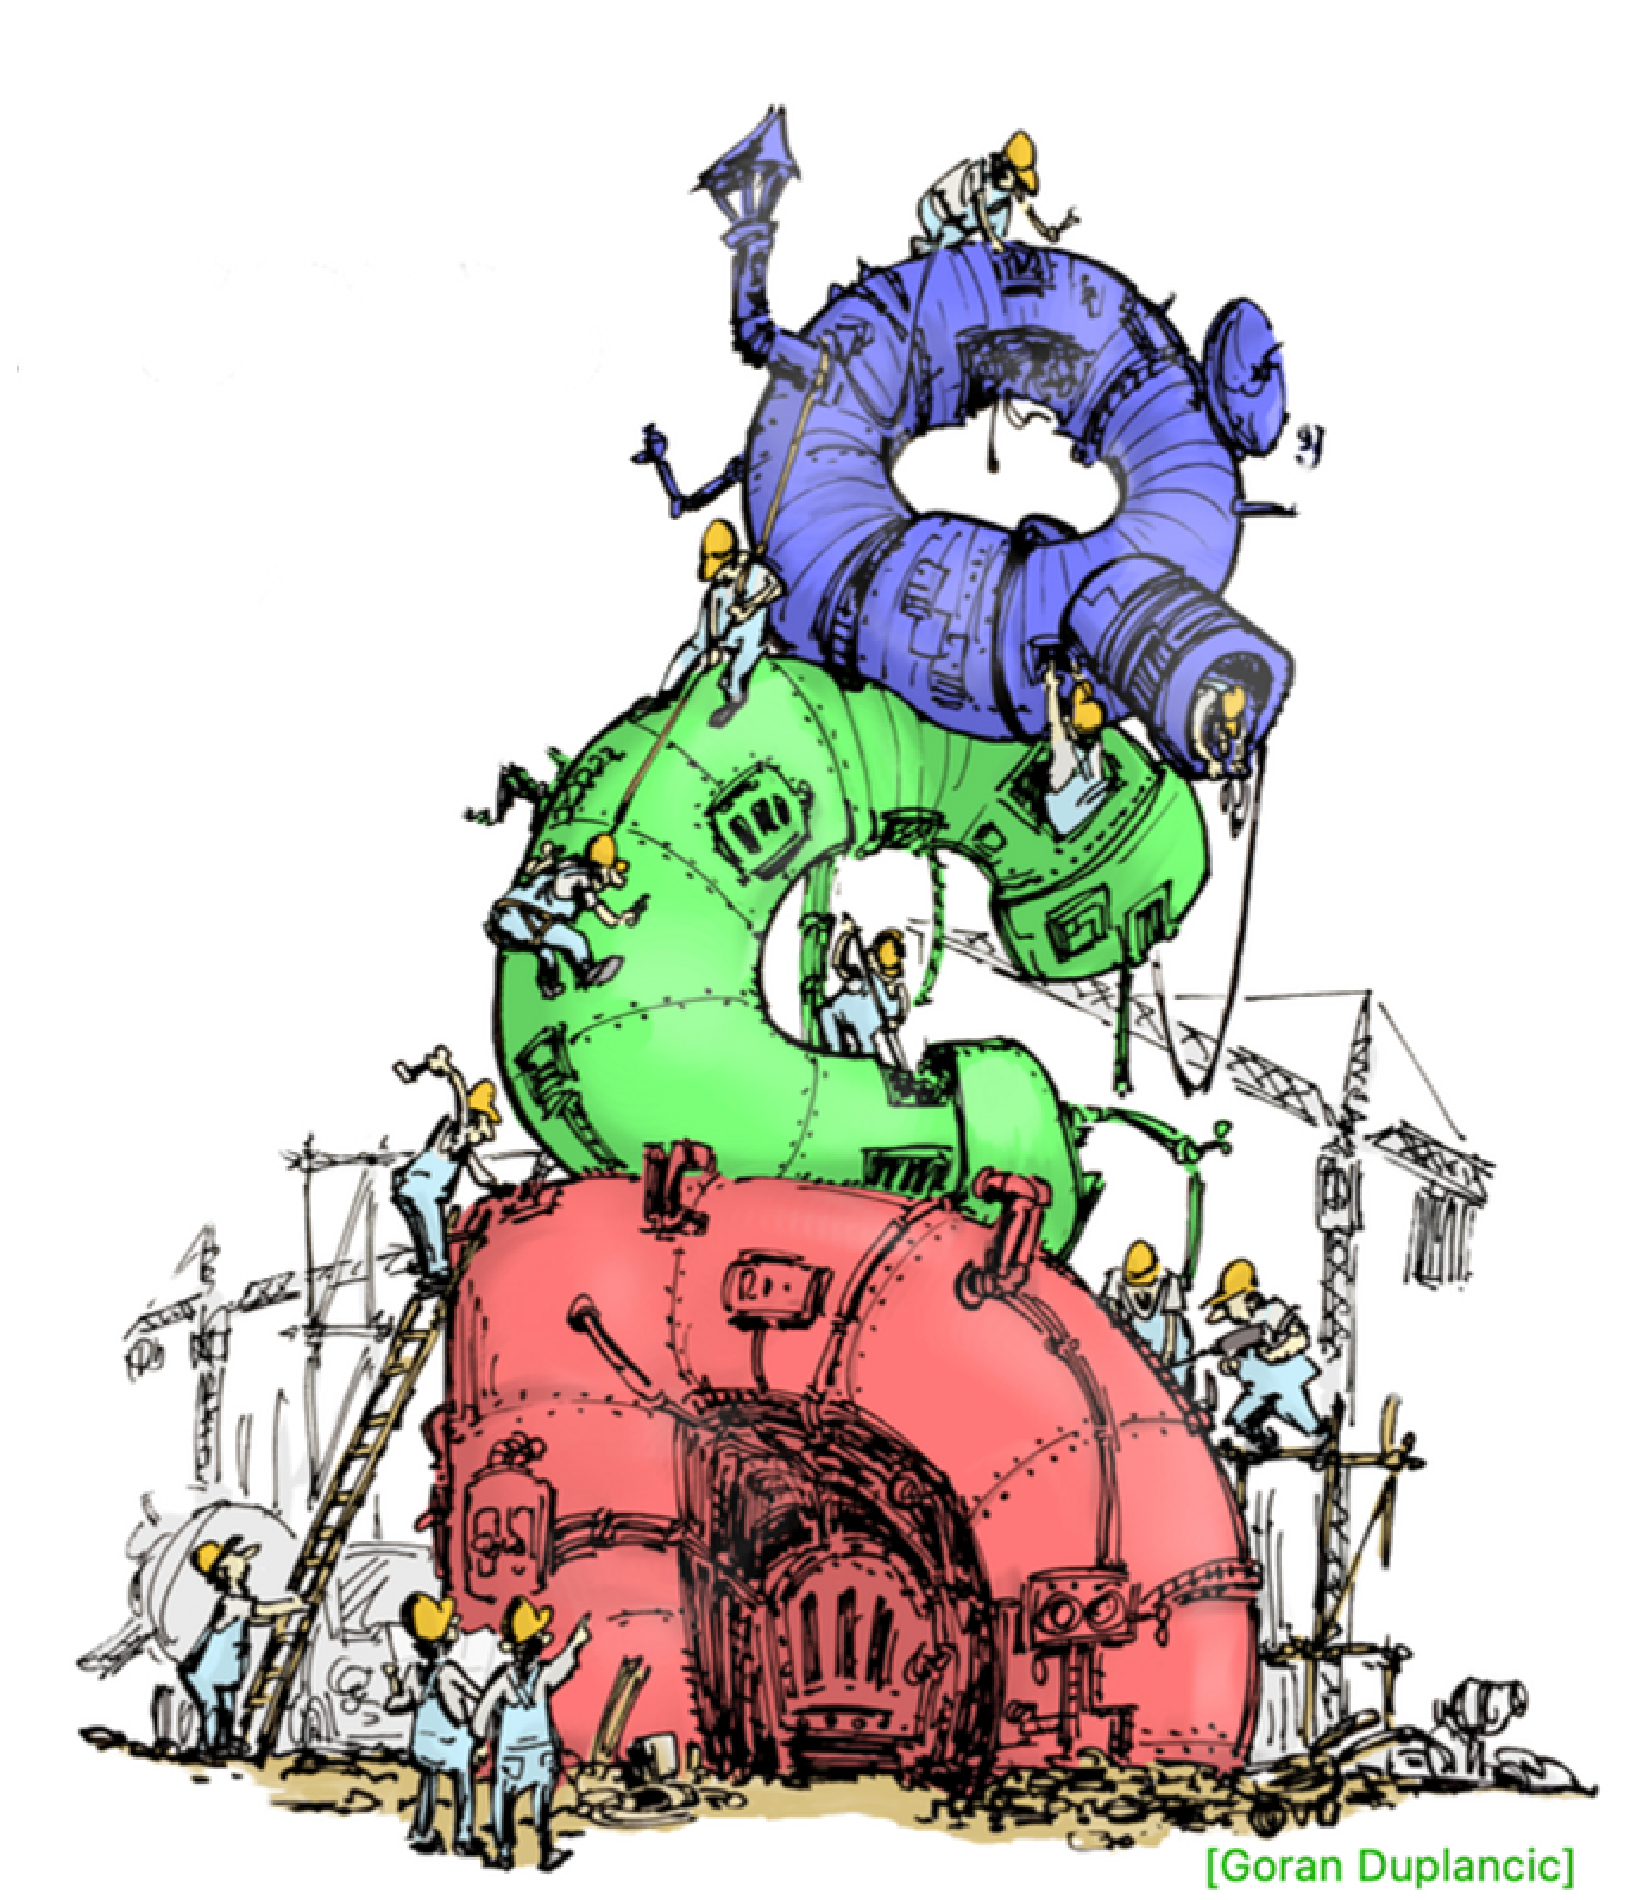
\includegraphics[scale=0.25]{sections/Chapters/Chapter1/Images/qcd.pdf}
    \caption{QCD is a colorful theory. A sketch by Goran Duplancic.}
\end{figure}

The QCD lagrangian is invariant under SU(3) color symmetry.

\begin{equation}
    \mathcal{L}_{QCD} = - \frac{1}{4} \sum_{a=1}^{8} F^a_{\mu \nu}F^{a \nu \mu} + \sum_{f=1}^{6} \overbar{\psi}_f^i
    (i \gamma^{\mu} (D_{\mu})_{ij} - m_f \delta_{ij}) \psi_f^j
\end{equation}


Let's discuss the indeces: $\mu$, $\nu$ are the usual Lorentz's indeces, $a$ is the gluon index, $f$ is the
flavour index, $i$ and $j$ are color indeces ($i$, $j = 1, 2, 3$).
Furthermore the lagrangian contains the Faraday's tensor and the covariant derivative:

\begin{align}
    &F^a_{\mu \nu} = \partial_{\nu} G^a_{\mu} - \partial_{\mu} G^a_{\nu} + g f^{abc}G_{\mu}^{b}G^c_{\nu} \\
    &(D_{\mu})_{ij} = \partial_{\mu} \delta_{ij} - i g \tau^a_{ij} G^a_{\mu}
\end{align}

where $f^{abc}$ are the structure's constant of the SU(3) group, $G^a_{\mu}$ is the gluon four-vector, 
$\tau^a$ are the SU(3) generators.

The main difference between the Strong and EW sector is that the spontaneous symmetry breaking 
mechanism is not necessary to describe quarks' masses, because the lagrangian's mass term is invariant 
under SU(3) symmetry.

\begin{figure}[h]
    \centering
    \includegraphics[scale=0.8]{sections/chapters/Chapter1/Images/Feynman_H_VV.pdf}
    \caption{Vertices of the SM. Top row: fermion-vector boson (Z, W, $\gamma$) interaction, gluon splitting, 
    (only for quarks), Yukawa coupling between Higgs and fermions.
    Middle row: Higgs couplings with two vector bosons and then a triple and 
    quadruple Higgs coupling. 
    Bottom row: triple and quadruple vector boson coupling and a HHVV coupling.}
\end{figure}


\begin{comment}

\subsection{Parton Model}


\subsection{Jets}

When studying high-energy collisions one often has to consider processes with gluons and quarks in the final state.
Quarks and gluons can be produced in numerous processes such as the decay of W, Z and H bosons.
However, these high-energy quarks and gluons are not directly observed in the final state of the collision.
They tend to undergo successive branchings at small angles, producing a series of collimated quarks and gluons. 
This cloud of collimated particle is often referred to as “parton shower".
The fact that this parton shower is collimated traces back to the collinear divergence of QCD.
Starting from a parton with high virtuality (of the order of the hard scale of the process), 
the parton shower will produce branchings into further partons of decreasing virtuality, 
until one reaches a non-perturbative (hadronisation) scale, typically of order $\Lambda_{QCD}$ ($\sim$ 1 GeV).
At this stage, due to confinement, these quarks and gluons will form hadrons.
Conceptually jets are collimated flows of hadrons.

\subsection{Jet algorithms}

After discussing the meaning and origin of jets in the introduction, we require an infrared-safe definition of 
jets. Historically, the first definition of a process with two jets was given by Sterman and Weinberg. 
They defined a process with two jets as a process in which it is possible to identify two cones of angle $\delta$, 
within which all the energy of the process is contained, with a discrepancy of at most $\epsilon$.
The Sterman-Weinberg's cross section has two equivalent definitions:

\begin{align}
    \sigma_{SW} &= \sigma^{q \bar{q}} + \sigma^{3 partons}(E_i < \epsilon \sqrt{s} \land \theta_{ij} < \delta) + \\
    + \sigma^{4 partons}(E_i < \epsilon \sqrt{s} \land \theta_{ij} < \delta) + ... \\
    &= \sigma^{tot} - \int_{R} \frac{\sigma^{tot}}{d x_1 d x_2}
\end{align}


The first definition defines the SW cross section as the sum of the cross sections with an increasing number 
of partons in the partonic final state. The cross section with two partons does not require any constraints 
since it naturally produces two jets. The cross section with three partons, in order to have two jets in the 
final state, requires constraints on the third parton, which must not form a jet. Hence, it must be either 
inside one of the cones ($\theta_{ij} < \delta$) or have an energy below the tolerance of $\epsilon \sqrt{s}$. 
Similarly, the cross section with four partons has the same constraints but on two partons instead of just one.

The second equivalent definition defines the SW cross section as the whole cross-section minus the hard 
cross-section.
The integration domain $R$ identifies the hard region of the Dalitz plot (i.e., the central one).


In the modern era the jet definitions are \textbf{jet algorithms} which are well-defined procedure that tells 
how to reconstruct the jets from the set of hadrons in the final state of the collision.
A jet algorithm has three main building blocks:

\begin{itemize}
    \item \textbf{Distance}.\\
    The distance expresses how much collinear or soft is an hadron.
    Therefore the definition of the distance plays a fundamental role to determine if an hadron lies within or
    outside a jet cone.
    The definition must be well-thought in order to avoid an unproper clustering procedure.
    \item \textbf{Cut}.\\
    The cut is the value that determines whether the hadron will be clustered to form a jet or not. 
    If it is too small, the algorithm would be too sensitive and would tend to identify a jet for each particle. 
    On the other hand, if it is too large, the algorithm tends to cluster every particle into a single jet.
    \item \textbf{Recombination Scheme}.\\
    The recombination scheme is the rule which builds the jet by recombining the four-momentum of particles
    that lie within the jet's cone.
    Examples of recombination schemes are the “E-scheme" and the “Winner Take All".
\end{itemize}

The workflow of a jet algorithm could be summarised by the flowchart shown in figure 
\end{comment}

\section{Quantum Computing in High Energy Physics}

The HEP and Quantum information communities have recently joined forces to investigate possible 
applications of Quantum Computing in High Energy Physics.
The recently published article by the QC4HEP Working Group \cite{dimeglio} summarizes these possible applications, which are divided in 
two main domain areas: theoretical methods and algorithms for modelling HEP problems, and numerical methods 
for the interpretation and analysis of experimental results (as well as detector simulation and event generation).\\
In the next two paragraphs I will briefly discuss this possible applications of QC to HEP.

\subsection{Quantum Computing for Theoretical Modelling in HEP}

Numerous theoretical simulations of lattice gauge theories rely on the widespread technique of euclidean 
path-integral Monte Carlo simulations.\\
However, this technique suffers from the \textit{sign problem}, which means that contributions 
to the path integral can cancel out, leading to numerical instability and increased computational cost.\\
Recently, Tensor Networks\footnote[1]{For an introduction on Tensor Networks \cite{Bridgeman_2017}.
For an introduction on the simulation of lattice gauge theories with Tensor Networks \cite{Dalmonte_2016}.} 
have become a popular alternative to circumvent the 
\textit{sign problem}.
Tensor Networks, which are based on the Hamiltonian formalism (as opposed to lattice gauge theory simulations 
that typically use the Lagrangian formalism), provide a powerful framework for efficiently parameterizing 
the \textit{physical corner} of a Hilbert space\footnote[2]{The physical corner of the Hilbert space is the 
subset that describes the low-energy states of a quantum system.}. 
This approach reduces the complexity of exploring the entire Hilbert space landscape by focusing on the 
relevant low-energy subspace.\\
A promising alternative to Tensor Networks are simulations on quantum computers, because the number of 
required qubit (the fundamental unit of information) grows linearly with the number of lattice sites.
In addition, by sharing with Tensor Networks the Hamiltonian formulation, quantum computations 
completely avoid the \textit{sign problem}.
Thus, quantum computers could be a potential framework to fully overcome the limitations 
outlined above for the simulation of lattice gauge theories and especially their real-time dynamics.


\subsection{Quantum Computing in HEP Experiments}

An experiment in HEP requires three different categories of algorithms:

\begin{enumerate}
    \item Detector operation.\\
    Detector operation algorithms allow detectors to efficiently obtain data that cleanly represents the 
    fundamental interactions of matter. Detectors like ATLAS and CMS feature very large amounts of very high 
    dimensional data, which requires algorithms that can handle such complex data.
    Moreover, these detectors require algorithms to sort significant signals from noise.
    \item Identification and reconstruction algorithms.\\
    Identification and reconstruction algorithms are an essential part of mapping the vast collection of 
    pixel intensities, timings, and event counts to a coherent underlying physics structure in the data.
    \item Simulation algorithms.\\
    Robust simulation and inference tools allow particle physics experiments to compare 
    large amounts of complex, highly structured data with parametrized theoretical predictions.
\end{enumerate}

Quantum Computing could play a fundamental role in each of the above-mentioned categories.\\
Experiments running on high-luminosity accelerators need faster algorithms and QC 
could be instrumental to speed-up the processing time of large datasets.
Moreover, quantum algorithms that leverage the unique properties of \textit{entanglement} and 
\textit{superposition} could potentially extract more information 
from a given dataset than classical algorithms.
Finally, quantum algorithms could capture more complex aspects of HEP theory and simulation providing 
estimators that are more natively aligned with the quantum mechanical nature of the Standard Model.

\begin{figure}
    \centering
    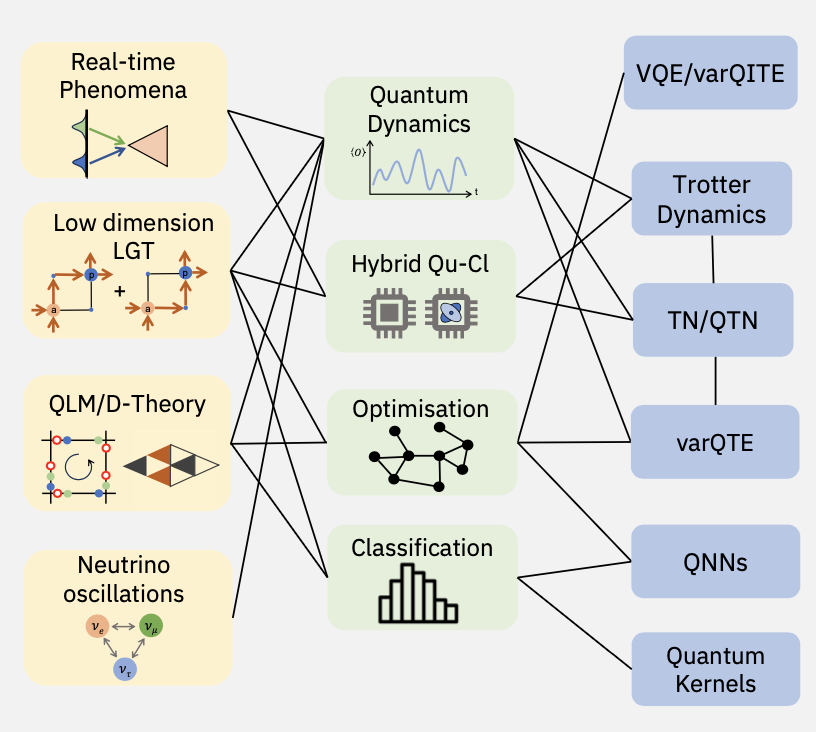
\includegraphics[scale=0.45]{sections/chapters/Chapter1/Images/exp-qc.png}
    \caption{In yellow, common High Energy Physics (HEP) tasks; in green, the corresponding machine 
    learning tasks; and in blue, the corresponding quantum algorithms.}
\end{figure}





